%%%%%%%%%%%%%%%%%%%%%%%%%%%%%%%%%%%%%%%%%%%%%%%%%%%%%%%%%%
% # Appendix: Reanalysis of Processing Data Results
%%%%%%%%%%%%%%%%%%%%%%%%%%%%%%%%%%%%%%%%%%%%%%%%%%%%%%%%%%

\chapter{Reanalysis of Processing Data Results}\label{app-results-reanalysis}

%========================================================%
\section{Resumption responses in the elicited production experiment}\label{app-ept-token-subgroup}
%========================================================%

% ORC Figure
% \begin{figure}
% \caption{Mean tokens by participant organized by subgroup in the ORC elicited production task} \label{fig:app-orc-ept-token-subgroup}
% \raggedright\setstretch{1}
% \includegraphics{../analysis/plots/orc_ept_token_subgroup2.png}
% \textit{Note}. Shading indicates 95\% $CI$s.
% \vspace{-12pt}
% \end{figure}

% SRC Figure
% \begin{figure}
% \caption{Mean tokens by participant organized by subgroup in the SRC elicited production task} \label{fig:app-src-ept-token-subgroup}
% \raggedright\setstretch{1}
% \includegraphics{../analysis/plots/src_ept_token_subgroup2.png}
% \textit{Note}. Shading indicates 95\% $CI$s.
% \vspace{-12pt}
% \end{figure}

% ORC Model
\begin{table}
\caption{Summary of mixed-effects logistic regression model on resumption rates for RP non-acceptors in the ORC elicited production task}\label{tab:app-orc-ept-token-subgroup-model}
\raggedright\setstretch{1}
\begin{tabularx}{\textwidth}{lrYYY}\toprule
Parameter & Estimate~($\hat{\beta}$) & \textit{SE} & $z$ & $p$ \\\midrule
\csvreader[late after line=\\,late after last line=\\\bottomrule]
{../analysis/tables/orc_ept_token_subgroup_model.csv}{}{\csvcoli & \csvcolii & \csvcoliii & \csvcoliv & \csvcolv}
\end{tabularx}
\textit{Note}. Model formula: Resumption \~{} Environment * Group + (1 | Participant) + (1 + Group | Item); reference level: Short + ENS; estimate unit: logit; intercept: grand mean.
\vspace{-12pt}
\end{table}

% ORC Posthoc
\begin{table}
\caption{Post-hoc tests for resumption rates for RP non-acceptors in the ORC elicited production task}\label{tab:app-orc-ept-token-subgroup-posthoc}
\raggedright\setstretch{1}
\begin{tabularx}{\textwidth}{lXYYYY}\toprule
Group & Contrast & Estimate~($\hat{\beta}$) & \textit{SE} & $z$ & $p$ \\\midrule
\csvreader[late after line=\\,late after last line=\\\bottomrule]
{../analysis/tables/orc_ept_token_subgroup_posthoc.csv}{}{\csvcoli & \csvcolii & \csvcoliii & \csvcoliv & \csvcolv & \csvcolvi}
\end{tabularx}
\textit{Note}. Adjustment to $p$-values done via multiple $t$ method for 9 tests.
\vspace{-12pt}
\end{table}

% SRC Model
\begin{table}
\caption{Summary of mixed-effects logistic regression model on resumption rates for RP non-acceptors in the SRC elicited production task}\label{tab:app-src-ept-token-subgroup-model}
\raggedright\setstretch{1}
\begin{tabularx}{\textwidth}{lrYYY}\toprule
Parameter & Estimate~($\hat{\beta}$) & \textit{SE} & $z$ & $p$ \\\midrule
\csvreader[late after line=\\,late after last line=\\\bottomrule]
{../analysis/tables/src_ept_token_subgroup_model.csv}{}{\csvcoli & \csvcolii & \csvcoliii & \csvcoliv & \csvcolv}
\end{tabularx}
\textit{Note}. Model formula: Resumption \~{} Environment * Group + (1 + Environment | Participant); reference level: Short + ENS; estimate unit: logit; intercept: grand mean.
\vspace{-12pt}
\end{table}

% SRC Posthoc
\begin{table}
\caption{Post-hoc tests for resumption rates for RP non-acceptors in the SRC elicited production task}\label{tab:app-src-ept-token-subgroup-posthoc}
\raggedright\setstretch{1}
\begin{tabularx}{\textwidth}{lXYYYY}\toprule
Group & Contrast & Estimate~($\hat{\beta}$) & \textit{SE} & $z$ & $p$ \\\midrule
\csvreader[late after line=\\,late after last line=\\\bottomrule]
{../analysis/tables/src_ept_token_subgroup_posthoc.csv}{}{\csvcoli & \csvcolii & \csvcoliii & \csvcoliv & \csvcolv & \csvcolvi}
\end{tabularx}
\textit{Note}. Adjustment to $p$-values done via multiple $t$ method for 3 tests.
\end{table}

%========================================================%
\section{Region-of-interest RTs in the self-paced reading experiment}\label{app-spr-rt-subgroup}
%========================================================%

% ORC Figure
% \begin{figure}
% \caption{Mean log RTs at Region 1 by subgroup in the ORC self-paced reading task} \label{fig:app-orc-spr-rt-subgroup}
% \raggedright\setstretch{1}
% 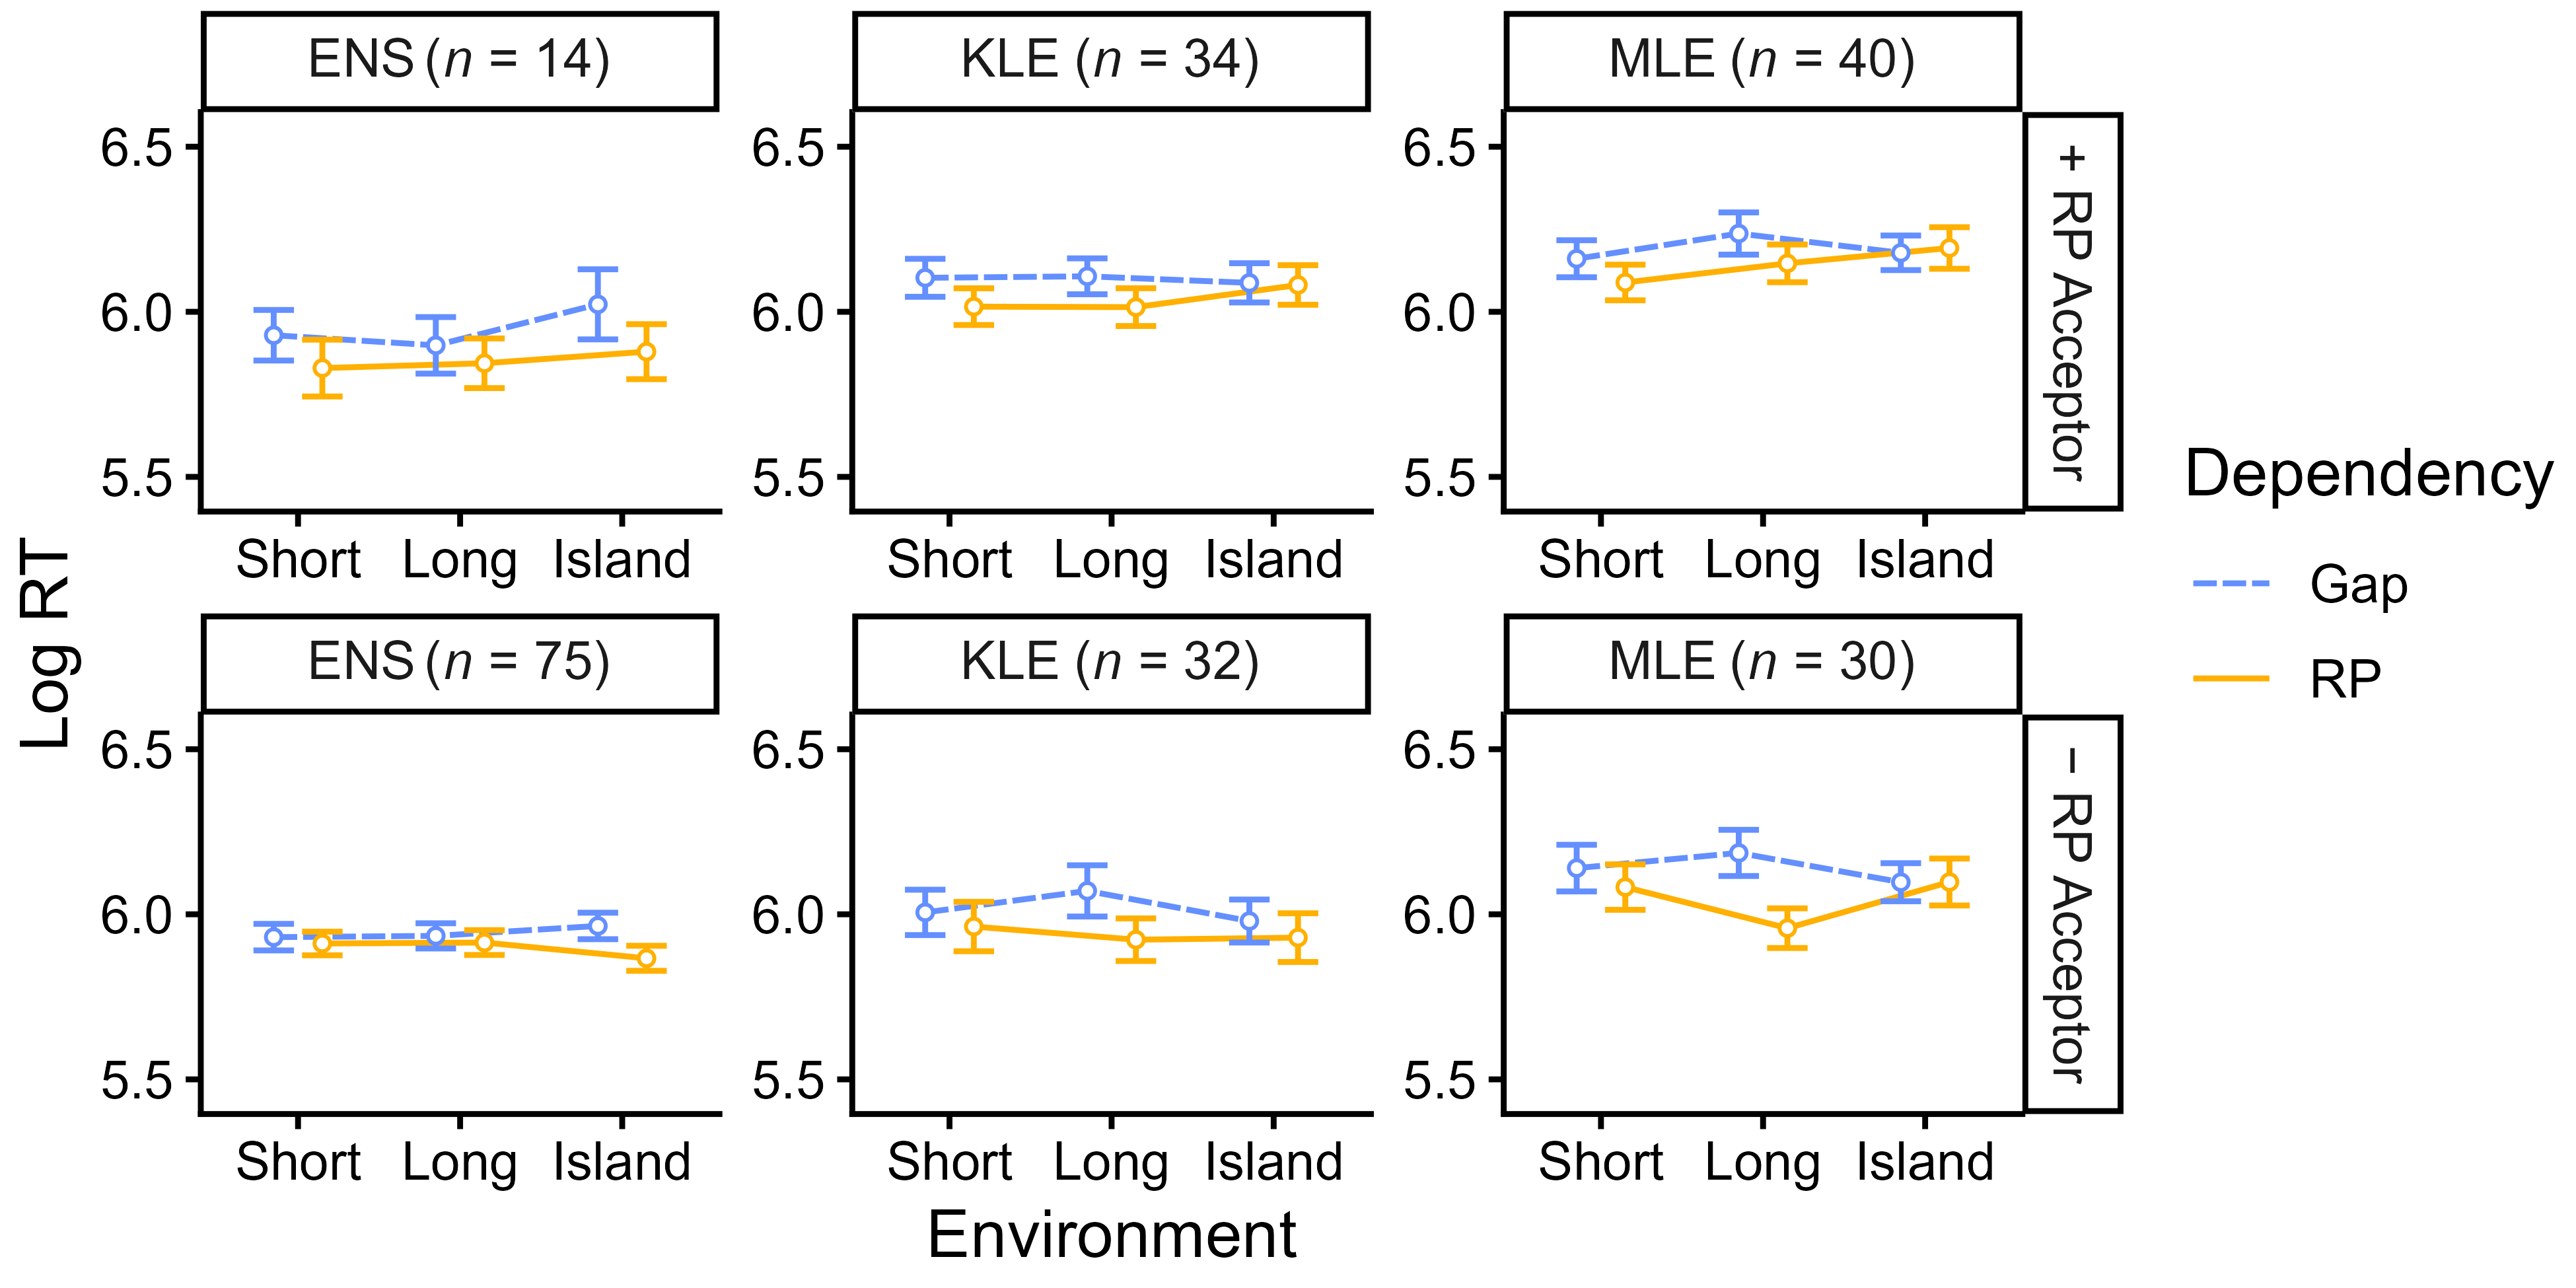
\includegraphics{../analysis/plots/orc_spr_rt_subgroup2.png}
% \textit{Note}. Shading indicates 95\% $CI$s.
% \vspace{-12pt}
% \end{figure}

% SRC Figure
% \begin{figure}
% \caption{Mean log RTs at Region 2 by subgroup in the SRC self-paced reading task} \label{fig:app-src-spr-rt-subgroup}
% \raggedright\setstretch{1}
% 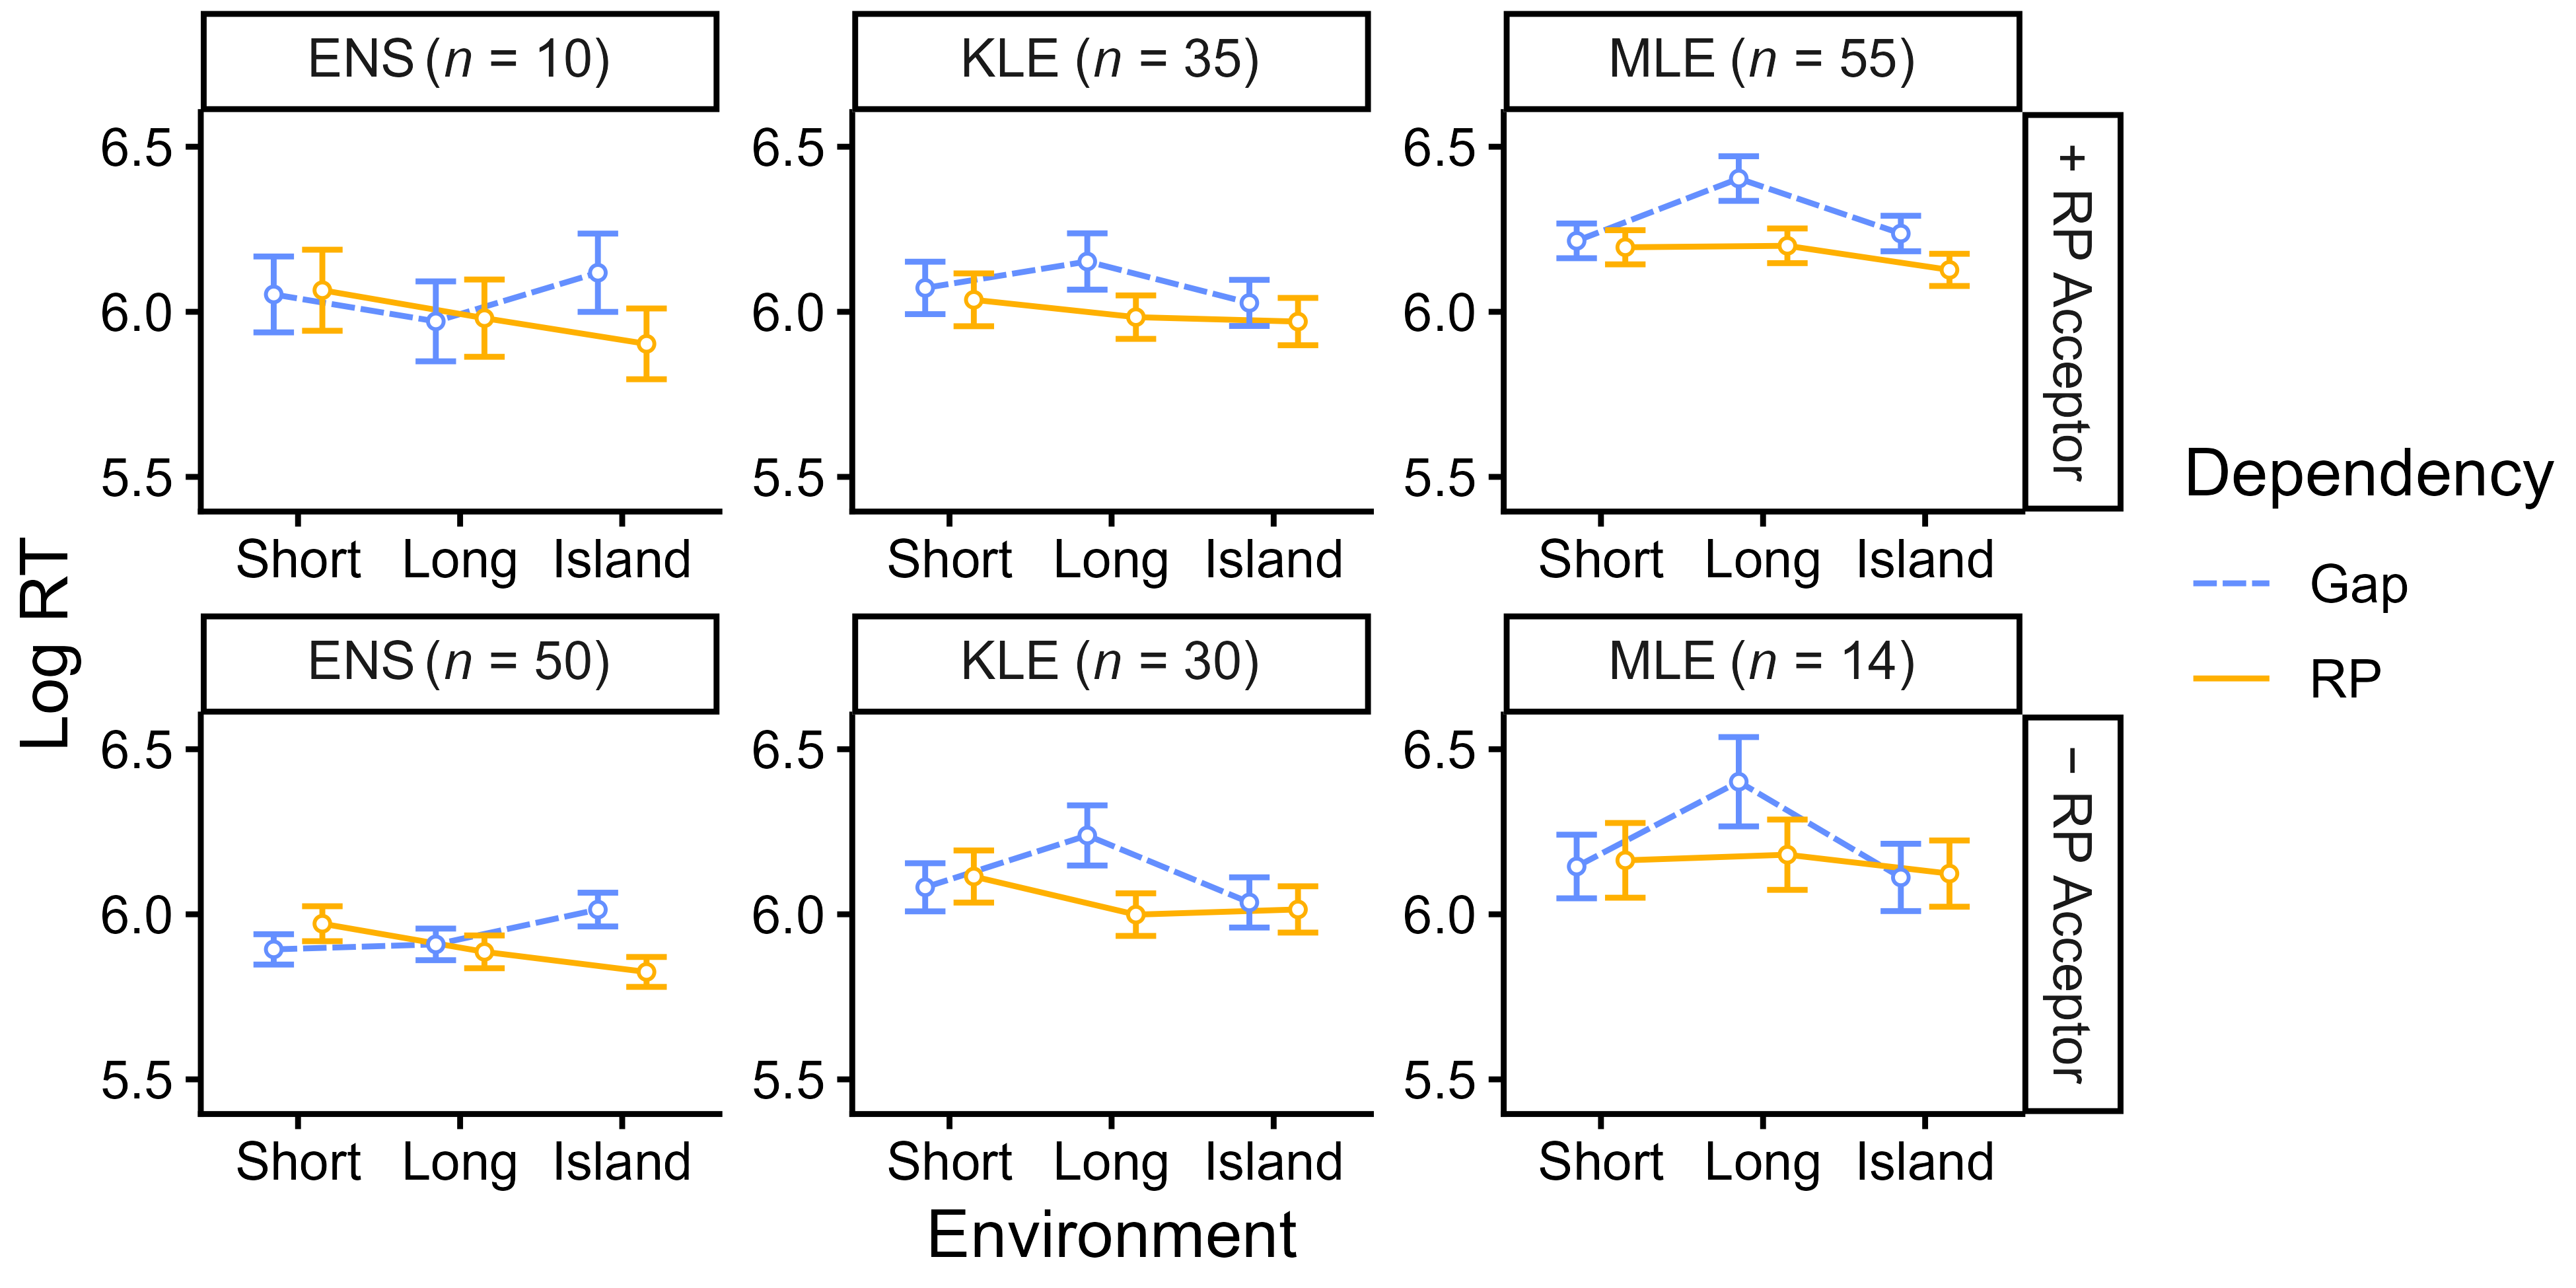
\includegraphics{../analysis/plots/src_spr_rt_subgroup2.png}
% \textit{Note}. Shading indicates 95\% $CI$s.
% \vspace{-12pt}
% \end{figure}

% ORC Model
\begin{table}
\caption{Summary of linear mixed-effects regression model on log RTs for RP non-acceptors in the ORC self-paced reading task}\label{tab:app-orc-spr-logrt-subgroup-model}
\raggedright\setstretch{1}
\begin{tabularx}{\textwidth}{lrYYY}\toprule
Parameter & Estimate~($\hat{\beta}$) & \textit{SE} & $z$ & $p$ \\\midrule
\csvreader[late after line=\\,late after last line=\\\bottomrule]
{../analysis/tables/orc_spr_logrt_subgroup_model.csv}{}{\csvcoli & \csvcolii & \csvcoliii & \csvcoliv & \csvcolv}
\end{tabularx}
\textit{Note}. Model formula: Log RT \~{} Dependency * Environment * Group + (1 + Dependency + Environment | Participant) + (1 + Dependency + Environment + Group | Item); reference level: Short + ENS; estimate unit: log-transformed millisecond; intercept: grand mean.
\vspace{-12pt}
\end{table}

% ORC Posthoc
\begin{table}
\caption{Post-hoc tests for log RTs of RP non-acceptors in the ORC self-paced reading task}\label{tab:app-orc-spr-logrt-subgroup-posthoc}
\raggedright\setstretch{1}
\begin{tabularx}{\textwidth}{lXXYYYY}\toprule
Group & Environment & Contrast & Estimate~($\hat{\beta}$) & \textit{SE} & $t$ & $p$ \\\midrule
\csvreader[late after line=\\,late after last line=\\\bottomrule]
{../analysis/tables/orc_spr_logrt_subgroup_posthoc.csv}{}{\csvcoli & \csvcolii & \csvcoliii & \csvcoliv & \csvcolv & \csvcolvi & \csvcolvii}
\end{tabularx}
\textit{Note}. Adjustment to $p$-values done via multiple $t$ method for 9 tests.
\vspace{-12pt}
\end{table}

% SRC Model
\begin{table}
\caption{Summary of linear mixed-effects regression model on log RTs for RP non-acceptors in the SRC self-paced reading task}\label{tab:app-src-spr-logrt-subgroup-model}
\raggedright\setstretch{1}
\begin{tabularx}{\textwidth}{lrYYY}\toprule
Parameter & Estimate~($\hat{\beta}$) & \textit{SE} & $z$ & $p$ \\\midrule
\csvreader[late after line=\\,late after last line=\\\bottomrule]
{../analysis/tables/src_spr_logrt_subgroup_model.csv}{}{\csvcoli & \csvcolii & \csvcoliii & \csvcoliv & \csvcolv}
\end{tabularx}
\textit{Note}. Model formula: Log RT \~{} Dependency * Environment * Group + (1 + Dependency + Environment | Participant) + (1 + Environment | Item); reference level: Short + ENS; estimate unit: log-transformed millisecond; intercept: grand mean.
\vspace{-12pt}
\end{table}

% SRC Posthoc
\begin{table}
\caption{Post-hoc tests for log RTs of RP non-acceptors in the SRC self-paced reading task}\label{tab:app-src-spr-logrt-subgroup-posthoc}
\raggedright\setstretch{1}
\begin{tabularx}{\textwidth}{lXXYYYY}\toprule
Group & Environment & Contrast & Estimate~($\hat{\beta}$) & \textit{SE} & $t$ & $p$ \\\midrule
\csvreader[late after line=\\,late after last line=\\\bottomrule]
{../analysis/tables/src_spr_logrt_subgroup_posthoc.csv}{}{\csvcoli & \csvcolii & \csvcoliii & \csvcoliv & \csvcolv & \csvcolvi & \csvcolvii}
\end{tabularx}
\textit{Note}. Adjustment to $p$-values done via multiple $t$ method for 9 tests.
\end{table}

%========================================================%
\section{Comprehension-question accuracy in the self-paced reading experiment}\label{app-spr-accuracy-subgroup}
%========================================================%

% ORC Figure
% \begin{figure}
% \caption{Mean comprehension-question accuracy by subgroup in the ORC self-paced reading task} \label{fig:app-orc-spr-accuracy-subgroup}
% \raggedright\setstretch{1}
% 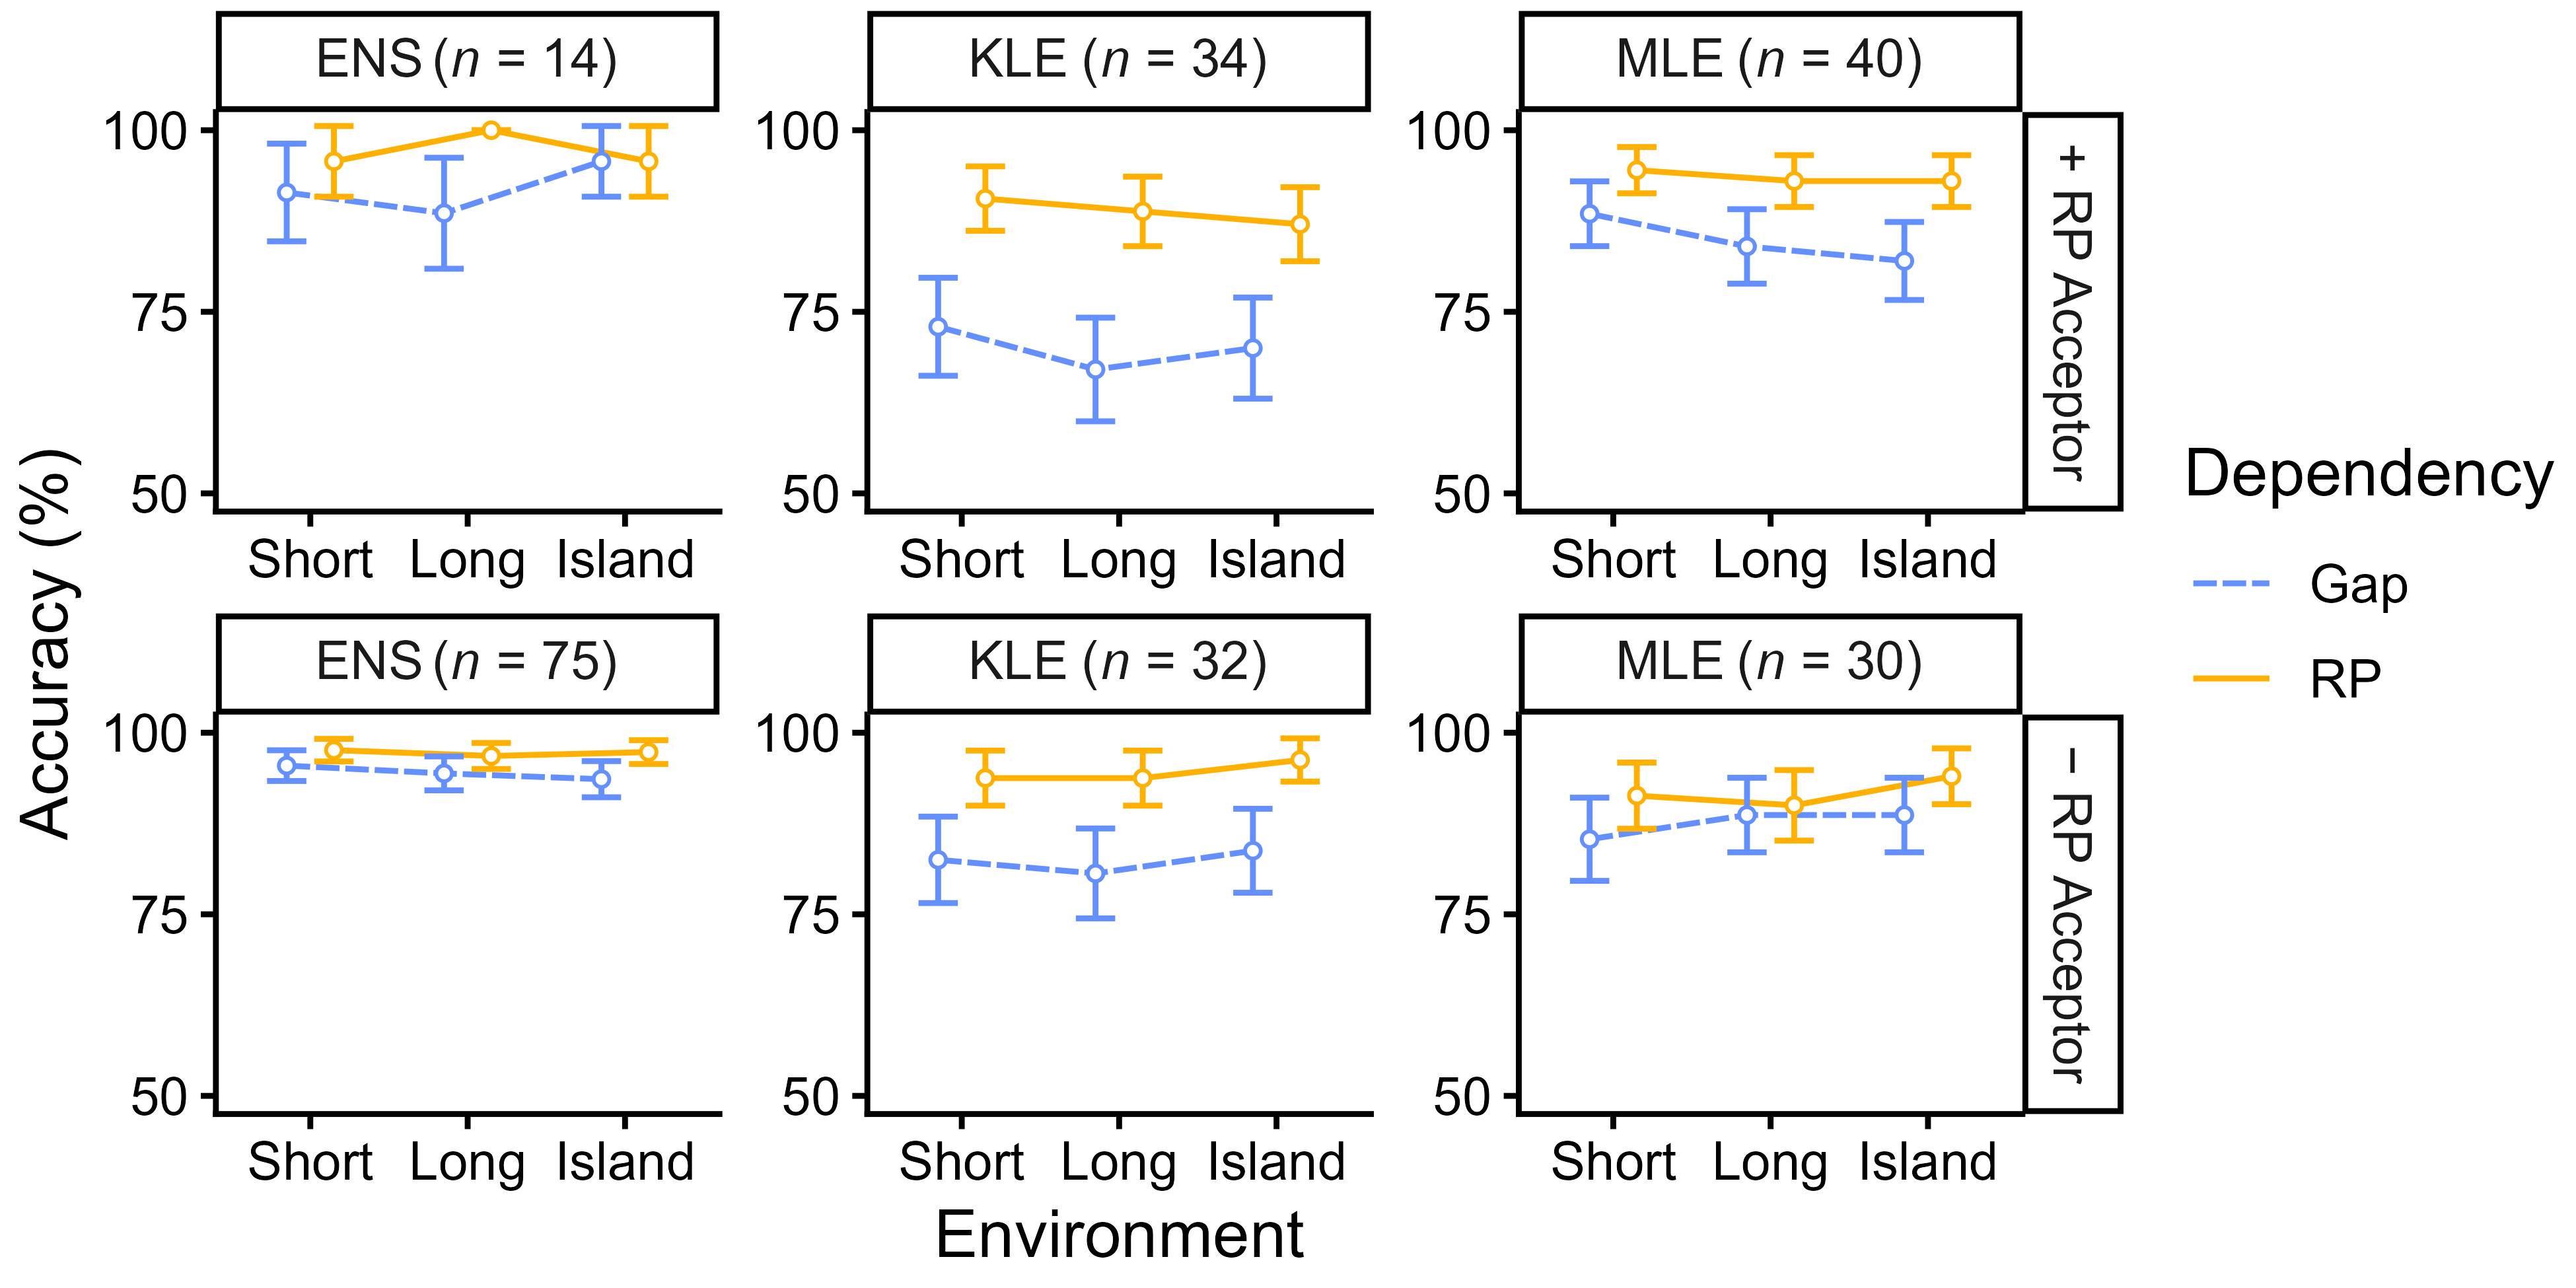
\includegraphics{../analysis/plots/orc_spr_accuracy_subgroup2.png}
% \textit{Note}. Error bars are 95\% $CI$s.
% \vspace{-12pt}
% \end{figure}

% SRC Figure
% \begin{figure}
% \caption{Mean comprehension-question accuracy by subgroup in the SRC self-paced reading task} \label{fig:app-src-spr-accuracy-subgroup}
% \raggedright\setstretch{1}
% 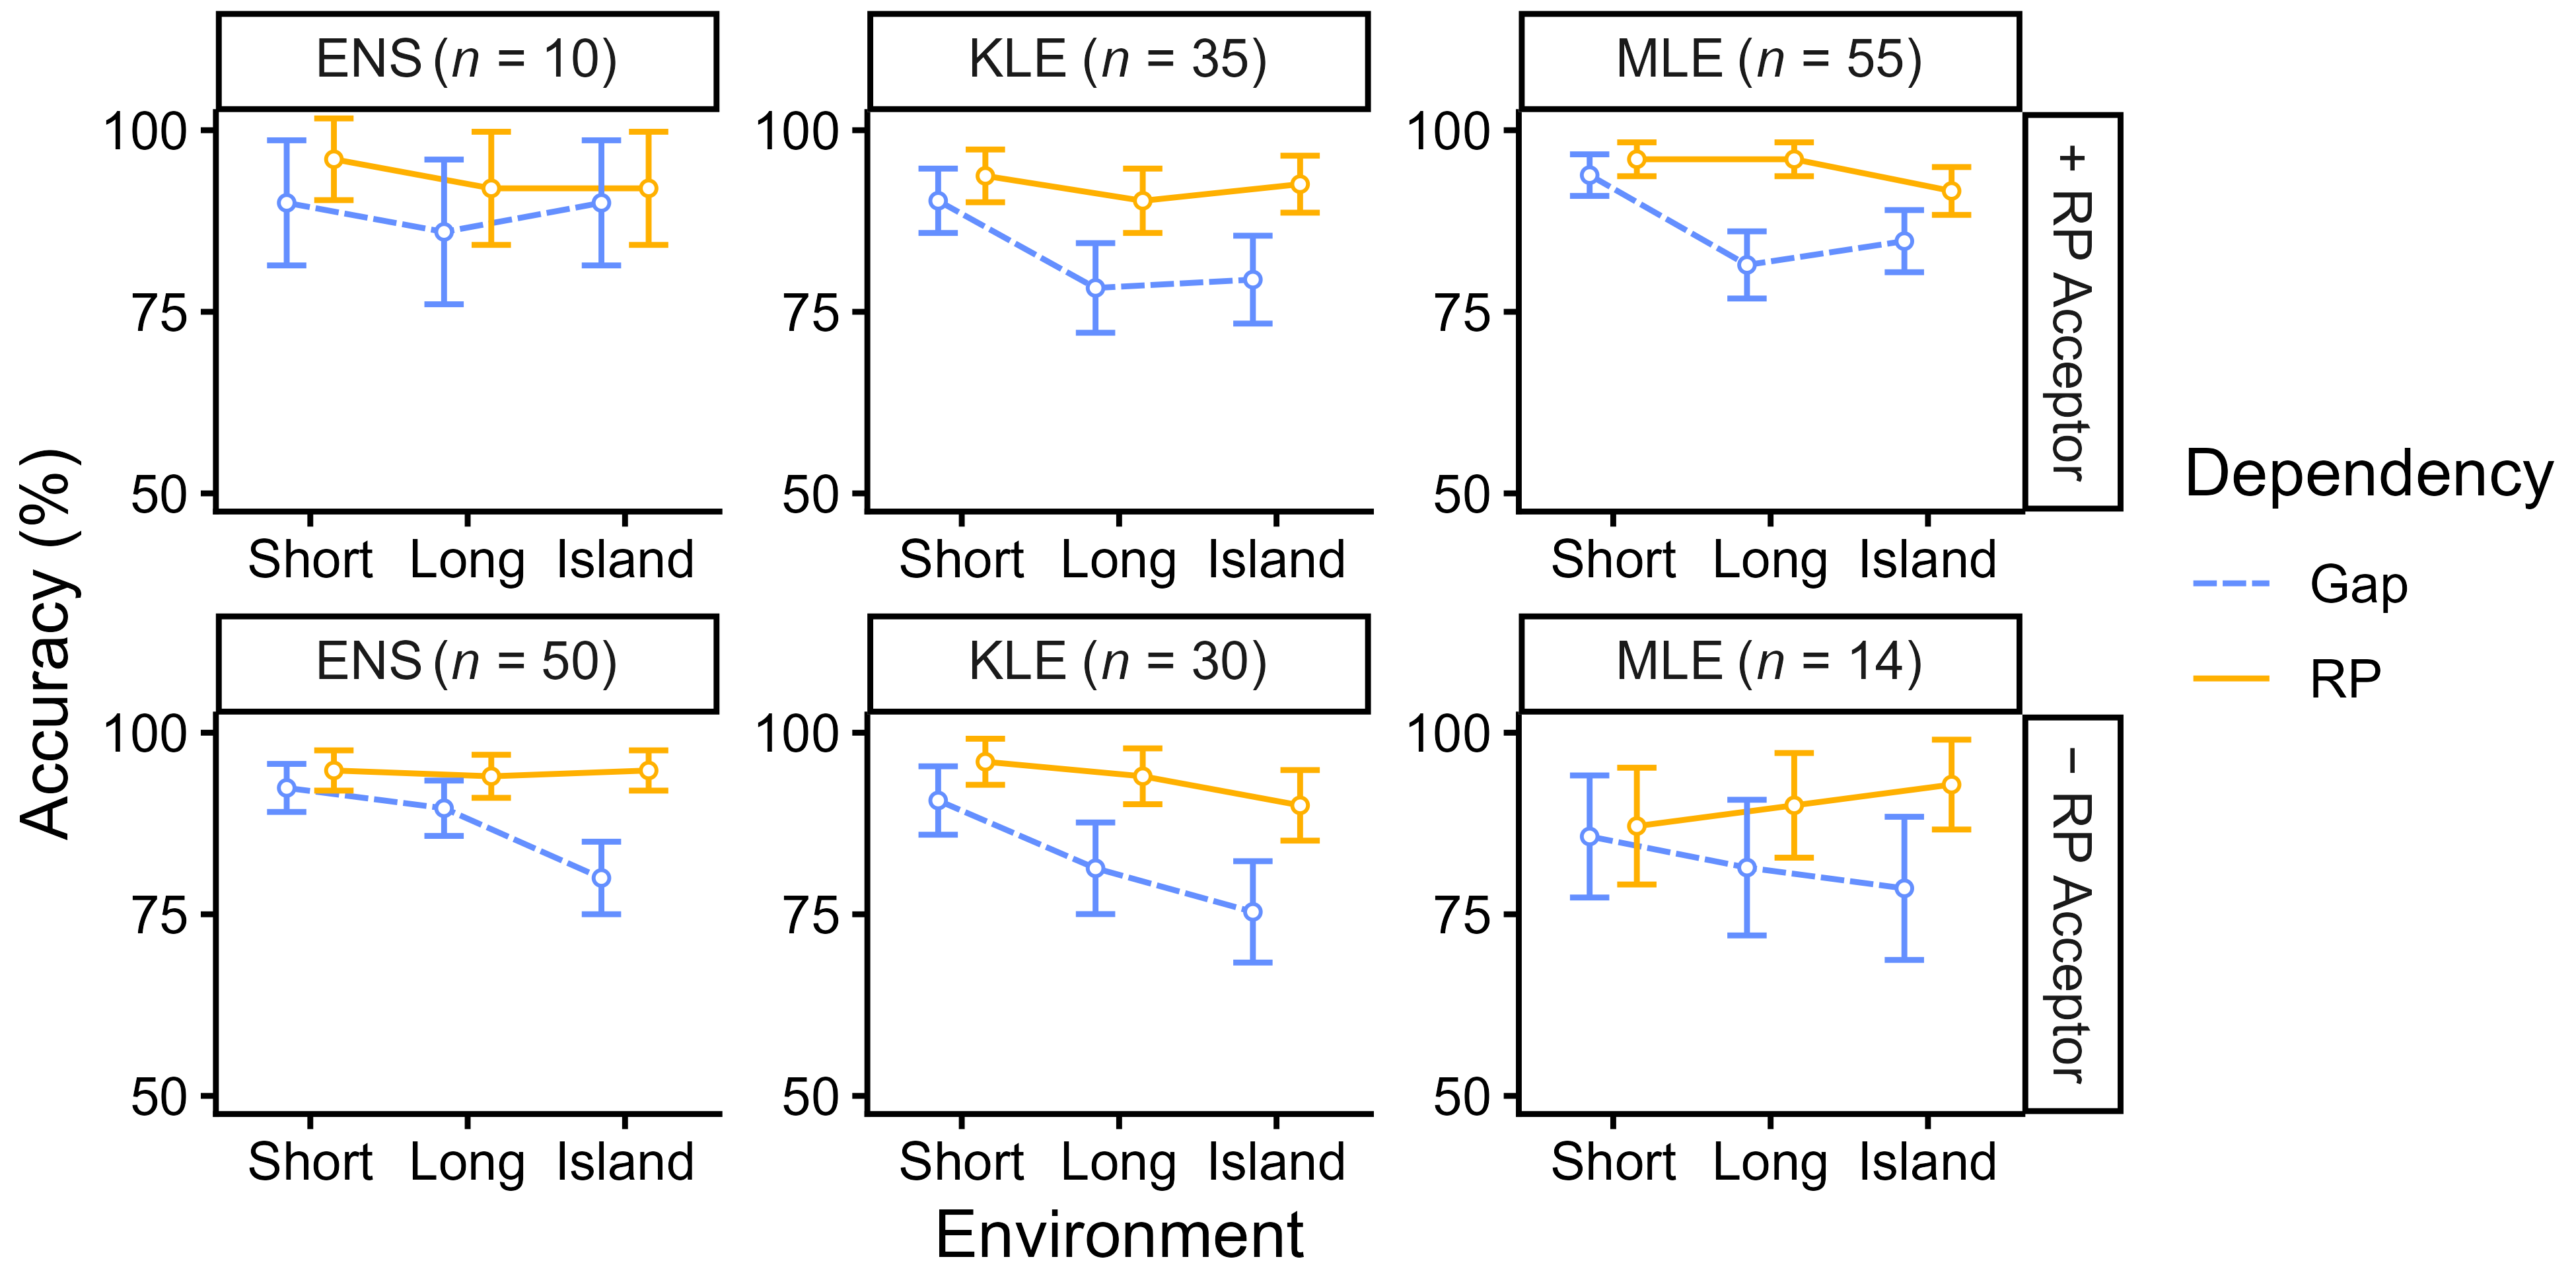
\includegraphics{../analysis/plots/src_spr_accuracy_subgroup2.png}
% \textit{Note}. Error bars are 95\% $CI$s.
% \vspace{-12pt}
% \end{figure}

% ORC Model
\begin{table}
\caption{Summary of linear mixed-effects regression model on comprehension-question accuracy for RP non-acceptors in the ORC self-paced reading task}\label{tab:app-orc-spr-accuracy-subgroup-model}
\raggedright\setstretch{1}
\begin{tabularx}{\textwidth}{lrYYY}\toprule
Parameter & Estimate~($\hat{\beta}$) & \textit{SE} & $z$ & $p$ \\\midrule
\csvreader[late after line=\\,late after last line=\\\bottomrule]
{../analysis/tables/orc_spr_accuracy_subgroup_model.csv}{}{\csvcoli & \csvcolii & \csvcoliii & \csvcoliv & \csvcolv}
\end{tabularx}
\textit{Note}. Model formula: Accuracy \~{} Dependency * Environment * Group + (1 + Dependency * Environment | Participant) + (1 + Dependency + Environment + Group | Item); reference level: Gap + Short + ENS; estimate unit: logit; intercept: grand mean.
\vspace{-12pt}
\end{table}

% ORC Posthoc
\begin{table}
\caption{Post-hoc tests for comprehension-question accuracy of RP non-acceptors in the ORC self-paced reading task}\label{tab:app-orc-spr-accuracy-subgroup-posthoc}
\raggedright\setstretch{1}
\begin{tabularx}{\textwidth}{lXXYYYY}\toprule
Group & Environment & Contrast & Estimate~($\hat{\beta}$) & \textit{SE} & $z$ & $p$ \\\midrule
\csvreader[late after line=\\,late after last line=\\\bottomrule]
{../analysis/tables/orc_spr_accuracy_subgroup_posthoc.csv}{}{\csvcoli & \csvcolii & \csvcoliii & \csvcoliv & \csvcolv & \csvcolvi & \csvcolvii}
\end{tabularx}
\textit{Note}. Adjustment to $p$-values done via multiple $t$ method for 9 tests.
\vspace{-12pt}
\end{table}

% SRC Model
\begin{table}
\caption{Summary of linear mixed-effects regression model on comprehension-question accuracy for RP non-acceptors in the SRC self-paced reading task}\label{tab:app-src-spr-accuracy-subgroup-model}
\raggedright\setstretch{1}
\begin{tabularx}{\textwidth}{lrYYY}\toprule
Parameter & Estimate~($\hat{\beta}$) & \textit{SE} & $z$ & $p$ \\\midrule
\csvreader[late after line=\\,late after last line=\\\bottomrule]
{../analysis/tables/src_spr_accuracy_subgroup_model.csv}{}{\csvcoli & \csvcolii & \csvcoliii & \csvcoliv & \csvcolv}
\end{tabularx}
\textit{Note}. Model formula: Accuracy \~{} Dependency * Environment * Group + (1 + Dependency * Environment | Participant) + (1 + Dependency + Environment + Group | Item); reference level: Gap + Short + ENS; estimate unit: logit; intercept: grand mean.
\vspace{-12pt}
\end{table}

% SRC Posthoc
\begin{table}
\caption{Post-hoc tests for comprehension-question accuracy of RP non-acceptors in the SRC self-paced reading task}\label{tab:app-src-spr-accuracy-subgroup-posthoc}
\raggedright\setstretch{1}
\begin{tabularx}{\textwidth}{lXXYYYY}\toprule
Group & Environment & Contrast & Estimate~($\hat{\beta}$) & \textit{SE} & $z$ & $p$ \\\midrule
\csvreader[late after line=\\,late after last line=\\\bottomrule]
{../analysis/tables/src_spr_accuracy_subgroup_posthoc.csv}{}{\csvcoli & \csvcolii & \csvcoliii & \csvcoliv & \csvcolv & \csvcolvi & \csvcolvii}
\end{tabularx}
\textit{Note}. Adjustment to $p$-values done via multiple $t$ method for 9 tests.
\vspace{-12pt}
\end{table}